\documentclass[11pt,a4paper]{article}

% =========================================================
% PACKAGES
% =========================================================
\usepackage[a4paper,margin=0.9in,headheight=15pt]{geometry}
\usepackage[T1]{fontenc}
\usepackage[utf8]{inputenc}
\usepackage{lmodern}
\usepackage{microtype}
\usepackage{graphicx}
\usepackage{float}
\usepackage{booktabs}
\usepackage{tabularx}
\usepackage{array}
\usepackage{enumitem}
\usepackage[table]{xcolor}
\usepackage{listings}
\usepackage{fancyhdr}
\usepackage{titlesec}
\usepackage{caption}
\usepackage{tikz}
\usetikzlibrary{arrows.meta,positioning,shapes.geometric}
\usepackage[most]{tcolorbox}
\usepackage{setspace}
\usepackage{hyperref}

\setstretch{1.08}
\setlength{\parskip}{4pt}
\setlength{\parindent}{0pt}

% =========================================================
% COLORS
% =========================================================
\definecolor{EricssonBlue}{RGB}{0,70,140}
\definecolor{DarkBlue}{RGB}{20,45,80}
\definecolor{LightBlue}{RGB}{235,243,252}
\definecolor{LightGray}{RGB}{247,247,247}
\definecolor{DarkGray}{RGB}{70,70,70}
\definecolor{PassGreen}{RGB}{22,120,60}
\definecolor{WarnAmber}{RGB}{176,110,0}
\definecolor{FailRed}{RGB}{170,40,40}

% =========================================================
% HYPERLINKS
% =========================================================
\hypersetup{
    colorlinks=true,
    linkcolor=EricssonBlue,
    urlcolor=EricssonBlue,
    citecolor=EricssonBlue,
    pdftitle={SecureTask - Technical Project and Security Assessment Report},
    pdfauthor={Parthak Bhardwaj}
}

% =========================================================
% PAGE STYLE
% =========================================================
\pagestyle{fancy}
\fancyhf{}
\lhead{\textcolor{EricssonBlue}{\textbf{SECURETASK}}}
\rhead{\textcolor{DarkGray}{Technical Project \& Security Assessment Report}}
\cfoot{\textcolor{DarkGray}{\thepage}}
\renewcommand{\headrulewidth}{0.5pt}
\renewcommand{\headrule}{\hbox to\headwidth{\color{EricssonBlue}\leaders\hrule height \headrulewidth\hfill}}

% =========================================================
% SECTION STYLE
% =========================================================
\titleformat{\section}
  {\Large\bfseries\color{DarkBlue}}
  {\thesection}{0.6em}{}
  [{\color{EricssonBlue}\titlerule[0.8pt]}]
\titleformat{\subsection}
  {\large\bfseries\color{EricssonBlue}}
  {\thesubsection}{0.6em}{}
\titlespacing*{\section}{0pt}{18pt}{8pt}
\titlespacing*{\subsection}{0pt}{12pt}{4pt}

\setlist{itemsep=1pt,topsep=3pt}
\captionsetup{font=small,labelfont={bf,color=EricssonBlue},skip=6pt}

% =========================================================
% CODE STYLE
% =========================================================
\lstset{
    basicstyle=\ttfamily\footnotesize,
    backgroundcolor=\color{LightGray},
    frame=single,
    rulecolor=\color{gray!40},
    breaklines=true,
    columns=fullflexible,
    showstringspaces=false,
    keywordstyle=\color{EricssonBlue}\bfseries,
    commentstyle=\color{DarkGray},
    xleftmargin=4pt,
    xrightmargin=4pt,
    aboveskip=6pt,
    belowskip=6pt
}

% =========================================================
% CUSTOM HELPERS
% =========================================================
\newcolumntype{L}[1]{>{\raggedright\arraybackslash}p{#1}}
\newcommand{\tablehead}{\rowcolor{LightBlue}}

\newcommand{\pass}{\textcolor{PassGreen}{\textbf{PASS}}}
\newcommand{\passcav}{\textcolor{WarnAmber}{\textbf{PASS (with caveats)}}}
\newcommand{\notdone}{\textcolor{FailRed}{\textbf{NOT PERFORMED}}}

% Callout box
\newtcolorbox{keybox}[1][Key Point]{
    enhanced, breakable,
    colback=LightBlue, colframe=EricssonBlue,
    fonttitle=\bfseries, title=#1,
    boxrule=0.6pt, arc=2pt,
    left=8pt, right=8pt, top=4pt, bottom=4pt
}

% Evidence figure: #1 path, #2 caption, #3 placeholder text
\newcommand{\evidence}[3]{%
  \begin{figure}[H]
    \centering
    \IfFileExists{#1}{%
        \includegraphics[width=0.88\textwidth,height=0.34\textheight,keepaspectratio]{#1}%
    }{%
        \fbox{\parbox[c][3.2cm][c]{0.85\textwidth}{\centering\color{DarkGray}[#3]\\[2pt]\footnotesize Place image at \texttt{#1}}}%
    }
    \caption{#2}
  \end{figure}%
}

% Flow diagram node style
\tikzset{
  flow/.style={draw=EricssonBlue, fill=LightBlue, rounded corners=3pt,
               minimum width=2.6cm, minimum height=1.0cm, align=center,
               font=\small\bfseries, text=DarkBlue},
  arr/.style={-{Stealth[length=2.5mm]}, thick, color=EricssonBlue}
}

% =========================================================
% DOCUMENT
% =========================================================
\begin{document}

% =========================================================
% COVER PAGE
% =========================================================
\begin{titlepage}
\centering
\vspace*{0.2cm}

% Place the official logo at logo/ericsson-logo.png (falls back to text if absent)
\IfFileExists{logo/ericsson-logo.png}{%
    \includegraphics[height=2.2cm,keepaspectratio]{logo/ericsson-logo.png}\par
}{%
    {\fontsize{30}{36}\selectfont\bfseries\textcolor{EricssonBlue}{Ericsson India Private Limited}\par}
}
\vspace{0.3cm}

\vspace{0.6cm}
\textcolor{EricssonBlue}{\rule{\textwidth}{1.5pt}}
\vspace{1.4cm}

{\fontsize{34}{40}\selectfont\bfseries\textcolor{DarkBlue}{SECURETASK}\par}
\vspace{0.4cm}
{\Large\textcolor{DarkGray}{Security-Focused Full-Stack Task Management Application}\par}

\vspace{1.4cm}
{\LARGE\bfseries Technical Project \& Security Assessment Report\par}

\vspace{1.6cm}
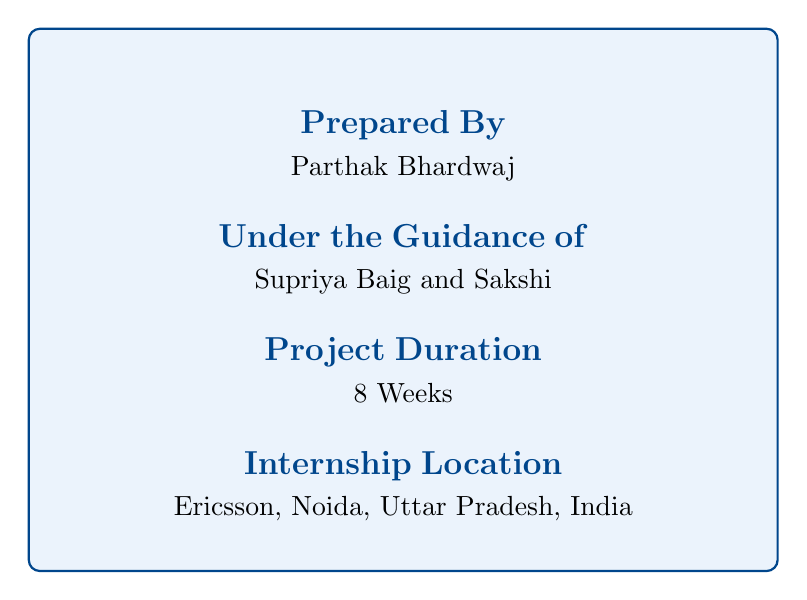
\begin{tikzpicture}
\node[draw=EricssonBlue, fill=LightBlue, line width=0.8pt, rounded corners=4pt,
      inner sep=18pt, text width=0.68\textwidth]{
\begin{center}
{\color{EricssonBlue}\textbf{\large Prepared By}}\\[3pt]
Parthak Bhardwaj\\[14pt]
{\color{EricssonBlue}\textbf{\large Under the Guidance of}}\\[3pt]
Supriya Baig and Sakshi\\[14pt]
{\color{EricssonBlue}\textbf{\large Project Duration}}\\[3pt]
8 Weeks\\[14pt]
{\color{EricssonBlue}\textbf{\large Internship Location}}\\[3pt]
Ericsson, Noida, Uttar Pradesh, India
\end{center}
};
\end{tikzpicture}

\vfill
{\large\textcolor{DarkGray}{Internship Project Report --- Completed at Ericsson, Noida, India}\par}
\vspace{0.2cm}
{\large\textcolor{DarkGray}{September 2026}\par}
\end{titlepage}

% =========================================================
% CONTENTS
% =========================================================
\pagenumbering{roman}
\tableofcontents
\clearpage
\listoffigures
\clearpage
\pagenumbering{arabic}

% =========================================================
% 1. EXECUTIVE SUMMARY
% =========================================================
\section{Executive Summary}

SecureTask is a security-focused full-stack task management application developed during an eight-week internship project. It provides user registration and login, JWT-based authentication and authorization, task CRUD operations, dashboard statistics, search and filtering, and a user profile.

The application is built with React, Flask, PostgreSQL, SQLAlchemy, JWT and bcrypt, and is deployed on Vercel, Render and Neon PostgreSQL.

Security was addressed throughout the project through manual testing, static analysis, secret scanning, dependency analysis, code-quality analysis and dynamic testing, using Bandit, Semgrep OSS, Gitleaks, OWASP Dependency-Check, pip-audit, Safety, SonarQube and OWASP ZAP.

\begin{keybox}[Headline Results]
\begin{itemize}[leftmargin=*]
\item \textbf{5 findings} identified and remediated: hardcoded test credential, Flask debug mode, permissive CORS, a vulnerable dependency, and missing bcrypt password-length validation.
\item \textbf{0 findings} in the final Bandit, Semgrep, Gitleaks, Dependency-Check, pip-audit and Safety scans.
\item \textbf{SonarQube:} 0 security vulnerabilities and Quality Gate passed (41 general issues remain).
\item \textbf{Not yet done:} a complete post-remediation OWASP ZAP active scan.
\end{itemize}
\end{keybox}

% =========================================================
% 2. PROJECT OVERVIEW
% =========================================================
\section{Project Overview}

\subsection{Objectives}
\begin{itemize}[leftmargin=*]
\item Develop a complete full-stack task management application.
\item Implement secure authentication and authorization, with passwords protected by bcrypt and sessions handled by JWT.
\item Implement task CRUD functionality.
\item Perform manual and automated security testing.
\item Identify and remediate security issues.
\item Deploy the application and document the security assessment.
\end{itemize}

\subsection{Main Features}
\begin{itemize}[leftmargin=*]
\item User registration and login
\item JWT authentication and protected routes
\item User-level authorization on all task operations
\item Task create, read, update and delete
\item Task search and category filtering
\item Dashboard statistics and user profile
\item Responsive user interface
\end{itemize}

% =========================================================
% 3. TECHNOLOGY STACK
% =========================================================
\section{Technology Stack}

\begin{table}[htbp]
\centering
\renewcommand{\arraystretch}{1.35}
\begin{tabularx}{\linewidth}{@{}L{0.26\linewidth}X@{}}
\toprule
\tablehead \textbf{Category} & \textbf{Technologies} \\
\midrule
Frontend & React.js, JavaScript, Tailwind CSS, Vite, React Router \\
HTTP Client & Axios \\
Backend & Python, Flask \\
Database & PostgreSQL, SQLAlchemy, psycopg2-binary \\
Authentication & JWT, Flask-JWT-Extended \\
Password Security & bcrypt \\
Cloud Services & Cloudinary \\
Version Control & Git, GitHub \\
Frontend Deployment & Vercel \\
Backend Deployment & Render \\
Database Hosting & Neon PostgreSQL \\
Security Testing & Bandit, Semgrep OSS, Gitleaks, OWASP Dependency-Check, pip-audit, Safety, SonarQube, OWASP ZAP \\
\bottomrule
\end{tabularx}
\caption{SecureTask technology stack}
\end{table}

% =========================================================
% 4. SYSTEM ARCHITECTURE
% =========================================================
\section{System Architecture}

SecureTask follows a client--server architecture with a clear separation between the presentation, application and data layers.

\begin{figure}[H]
\centering
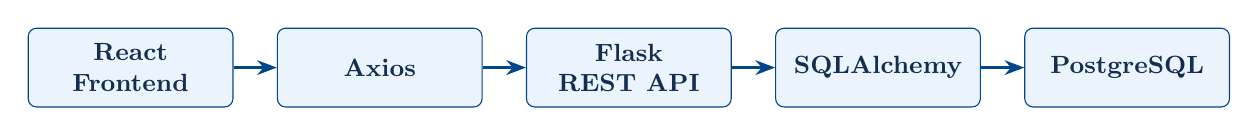
\begin{tikzpicture}[node distance=0.55cm]
\node[flow] (a) {React\\Frontend};
\node[flow, right=of a] (b) {Axios};
\node[flow, right=of b] (c) {Flask\\REST API};
\node[flow, right=of c] (d) {SQLAlchemy};
\node[flow, right=of d] (e) {PostgreSQL};
\draw[arr] (a)--(b);
\draw[arr] (b)--(c);
\draw[arr] (c)--(d);
\draw[arr] (d)--(e);
\end{tikzpicture}
\caption{High-level application architecture}
\end{figure}

\subsection{Frontend Layer}
The frontend handles the user interface, authentication screens, task management, dashboard, profile, search and filtering, protected routes and all API communication.

\subsection{Backend Layer}
The Flask backend exposes REST APIs for user registration, authentication, JWT validation, task management, authorization and database operations.

\subsection{Database Layer}
PostgreSQL stores application data, while SQLAlchemy provides the ORM layer between the Flask application and the database.

% =========================================================
% 5. AUTHENTICATION AND AUTHORIZATION
% =========================================================
\section{Authentication and Authorization}

\subsection{Authentication Flow}
SecureTask uses JWT-based authentication with Flask-JWT-Extended.

\begin{enumerate}[leftmargin=*]
\item The user registers an account.
\item The password is hashed with bcrypt and the hash is stored in PostgreSQL.
\item The user logs in with their credentials.
\item bcrypt verifies the password against the stored hash.
\item The backend generates a JWT.
\item The JWT is sent with every protected API request.
\end{enumerate}

Authenticated requests use the \texttt{Authorization} header, and the backend validates the token before granting access to protected endpoints:

\begin{lstlisting}
Authorization: Bearer <JWT>
\end{lstlisting}

\subsection{Authorization}
Authorization determines what an authenticated user may access. SecureTask enforces it through:

\begin{itemize}[leftmargin=*]
\item Protected Flask API routes and JWT validation
\item User-specific resource checks on task operations
\item React protected routes on the client
\end{itemize}

Together these prevent users from reaching resources that belong to other users through unauthorized requests.

\subsection{Password Security}
Passwords are never stored as plaintext. bcrypt hashes passwords at registration and verifies them at login.

% =========================================================
% 6. SECURITY IMPLEMENTATION
% =========================================================
\section{Security Implementation}

\subsection{JWT Secret Management}
Sensitive configuration, including the JWT secret, is supplied through environment variables rather than hardcoded in the source code.

\subsection{CORS Security}
An explicit allowlist of trusted origins replaces the earlier permissive configuration:

\begin{lstlisting}[language=Python]
ALLOWED_ORIGINS = [
    "https://secure-task-chi.vercel.app",
    "http://localhost:5173",
    "http://127.0.0.1:5173"
]

CORS(
    app,
    resources={r"/*": {"origins": ALLOWED_ORIGINS}}
)
\end{lstlisting}

Both trusted and untrusted origins were tested to verify the behavior (see Figures~\ref{fig:cors-ok} and~\ref{fig:cors-bad}).

\subsection{Input Validation}
Validation was added for security-sensitive inputs. A specific check was implemented for passwords because bcrypt only processes the first 72 bytes of its input.

% =========================================================
% 7. SECURITY TESTING METHODOLOGY
% =========================================================
\section{Security Testing Methodology}

The assessment combined several complementary approaches:

\begin{itemize}[leftmargin=*]
\item Manual application security testing
\item Static Application Security Testing (SAST)
\item Secret scanning
\item Dependency vulnerability scanning
\item Code-quality and security analysis
\item Dynamic Application Security Testing (DAST)
\end{itemize}

\subsection{Manual Security Tests}
The following scenarios were tested manually:

\begin{itemize}[leftmargin=*]
\item SQL injection
\item Cross-site scripting (XSS)
\item Authentication bypass
\item IDOR / authorization
\item Password hashing
\item Invalid task IDs
\item Malformed JSON
\item Verbose error handling
\end{itemize}

Directory traversal and file upload testing were considered not applicable because the application does not implement that functionality.

% =========================================================
% 8. SECURITY TOOLS AND RESULTS
% =========================================================
\section{Security Tools and Results}

\begin{table}[htbp]
\centering
\renewcommand{\arraystretch}{1.4}
\begin{tabularx}{\linewidth}{@{}L{0.26\linewidth}X@{}}
\toprule
\tablehead \textbf{Tool} & \textbf{Result / Purpose} \\
\midrule
Bandit & Python security static analysis. Final: High 0, Medium 0, Low 0. \\
Semgrep OSS & 459 rules, 46 targets, 0 findings. \\
Gitleaks & 17 commits scanned, 0 leaks. \\
OWASP Dependency-Check & 150 dependencies scanned; 0 vulnerable dependencies after remediation. \\
pip-audit & No known vulnerabilities in the specified requirements file. \\
Safety & 0 vulnerabilities in the requirements-file check. \\
SonarQube & 0 security vulnerabilities; Quality Gate passed; 41 total issues remain. \\
OWASP ZAP & 3,465 requests, 86 alert instances, 19 distinct alert types. Findings were manually triaged. \\
\bottomrule
\end{tabularx}
\caption{Security assessment results by tool}
\end{table}

% =========================================================
% 9. VULNERABILITIES AND REMEDIATION
% =========================================================
\section{Vulnerabilities and Remediation}

\begin{table}[htbp]
\centering
\renewcommand{\arraystretch}{1.45}
\begin{tabularx}{\linewidth}{@{}L{0.30\linewidth}X@{}}
\toprule
\tablehead \textbf{Finding} & \textbf{Remediation} \\
\midrule
Hardcoded test secret & Removed the secret and moved sensitive configuration to environment variables. \\
Flask debug configuration & Debug mode disabled. \\
Permissive CORS & Replaced with an explicit trusted-origin allowlist. \\
Vulnerable \texttt{nanoid} dependency & Updated from \texttt{3.3.17} to \texttt{3.3.18}. \\
Bcrypt password-length issue & Added UTF-8 byte-length validation before passwords reach bcrypt. \\
\bottomrule
\end{tabularx}
\caption{Security findings and remediation}
\end{table}

% =========================================================
% 10. OWASP ZAP ASSESSMENT
% =========================================================
\section{OWASP ZAP Assessment}

OWASP ZAP was used for dynamic testing against the local application:

\begin{itemize}[leftmargin=*]
\item Frontend: \texttt{http://localhost:5173}
\item Backend: \texttt{http://127.0.0.1:5000}
\end{itemize}

The active scan generated 3,465 requests, 86 alert instances and 19 distinct alert types. Alert instances are not equivalent to confirmed unique vulnerabilities, so each was manually triaged.

\subsection{Bcrypt Password-Length Finding}

ZAP reported password-related observations classified as \emph{Buffer Overflow} and \emph{Format String Error}. Manual reproduction with an oversized password produced an HTTP~500 response. Investigation traced this to bcrypt's 72-byte password limit rather than to a memory-safety flaw.

The application was updated to validate the password byte length:

\begin{lstlisting}[language=Python]
if len(password.encode("utf-8")) > 72:
    return jsonify({
        "message": "Password must be 72 bytes or fewer"
    }), 400
\end{lstlisting}

After remediation, the same oversized password returned HTTP~400 without exposing a traceback.

\begin{keybox}[Conclusion of the Investigation]
The ZAP alert labels were treated as scanner classifications. The confirmed root cause was missing bcrypt input validation, now fixed and verified.
\end{keybox}

% =========================================================
% 11. SCREENSHOTS AND EVIDENCE
% =========================================================
\clearpage
\section{Screenshots and Security Evidence}

This section presents selected screenshots of the application and of the main security activities. The complete evidence set is maintained in:

\begin{lstlisting}
docs/security/evidence/
\end{lstlisting}

\subsection{Application Screens}
\evidence{screenshots/login.png}{SecureTask login screen}{Login Screenshot}
\evidence{screenshots/dashboard.png}{SecureTask dashboard}{Dashboard Screenshot}
\evidence{screenshots/tasks.png}{SecureTask task management interface}{Task Management Screenshot}

\subsection{Security Tool Evidence}
\evidence{security/evidence/04-bandit-rescan.png}{Bandit final security scan}{Bandit Final Scan}
\evidence{security/evidence/08-sonarqube-rescan.png}{SonarQube final security and code-quality analysis}{SonarQube Final Analysis}
\evidence{security/evidence/22-gitleaks-final-scan.png}{Gitleaks repository secret scan}{Gitleaks Final Scan}
\evidence{security/evidence/24-dependency-check-rescan.png}{OWASP Dependency-Check final scan}{Dependency-Check Final Scan}

\subsection{CORS Verification}
\begin{figure}[H]
  \centering
  \IfFileExists{security/evidence/09-trusted-origin.png}{%
    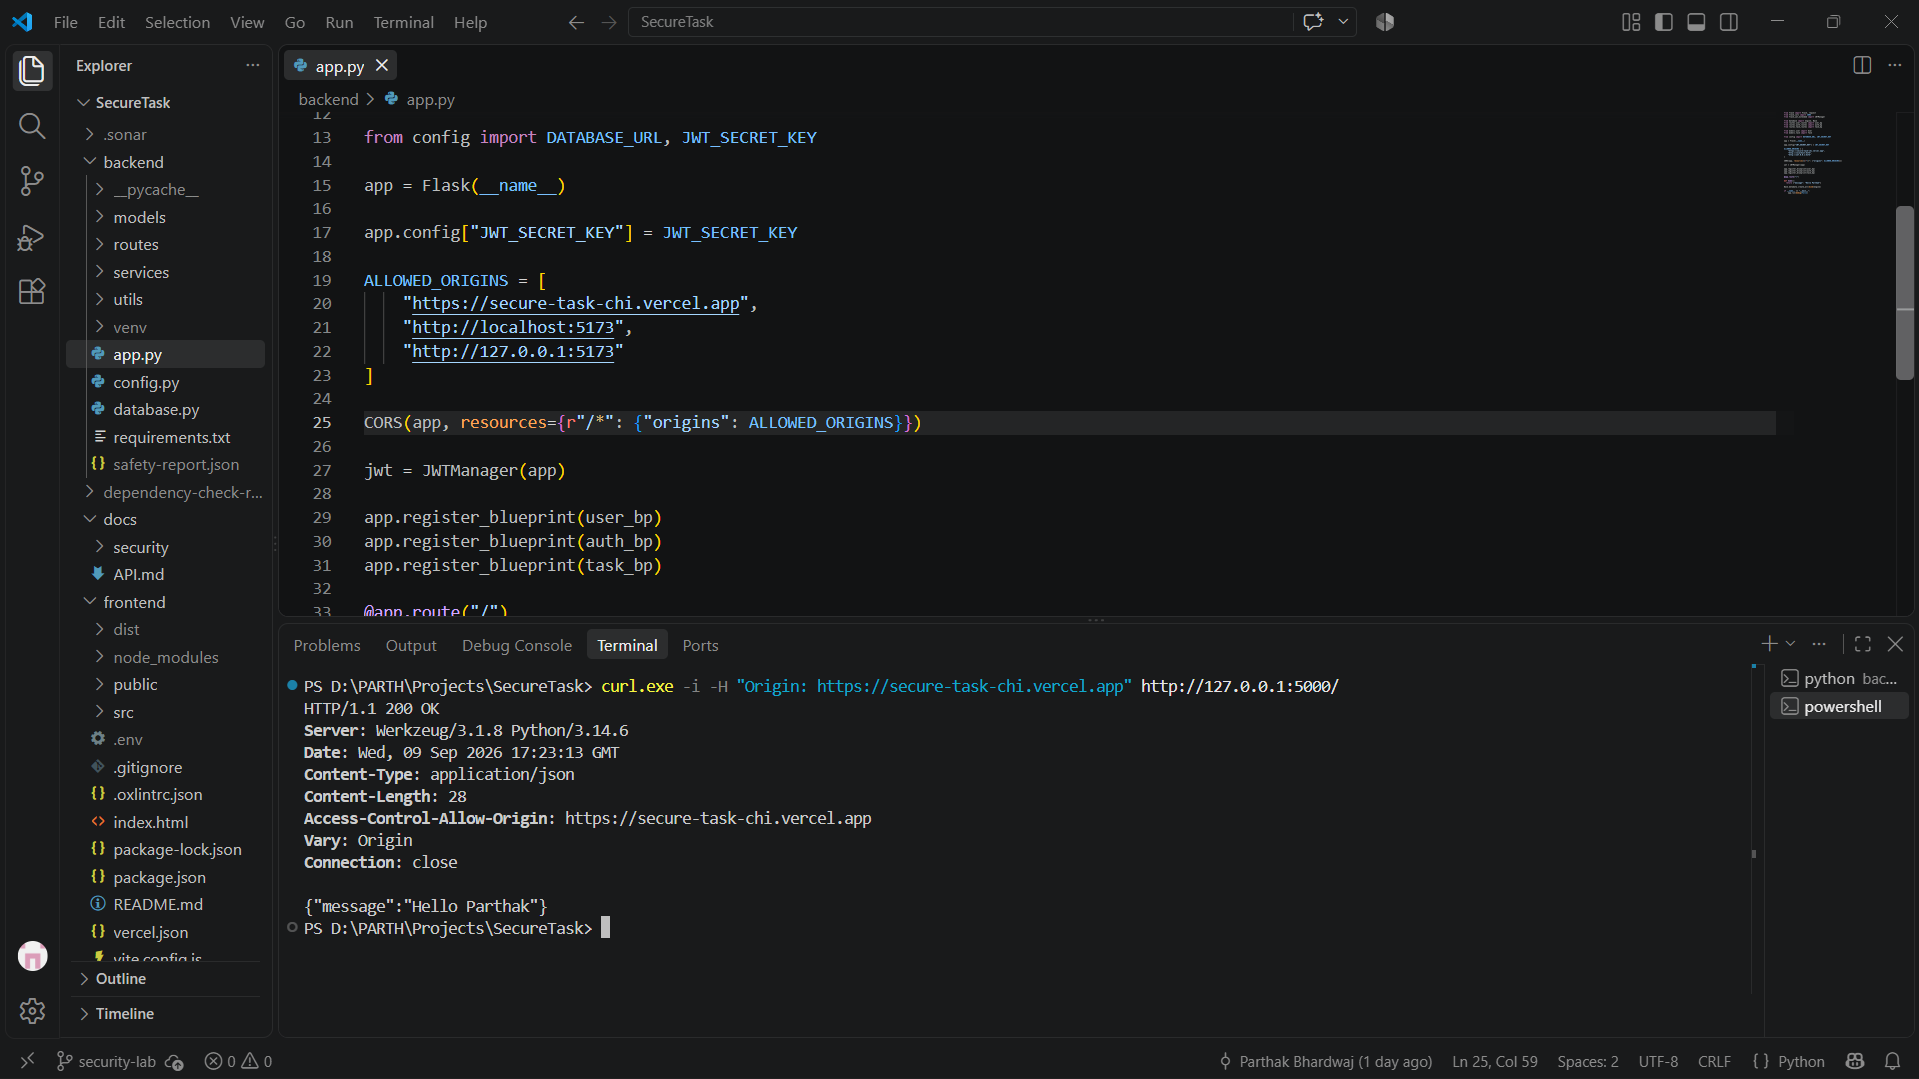
\includegraphics[width=0.88\textwidth,height=0.34\textheight,keepaspectratio]{security/evidence/09-trusted-origin.png}}{%
    \fbox{\parbox[c][3.2cm][c]{0.85\textwidth}{\centering\color{DarkGray}[Trusted Origin Test]}}}
  \caption{Trusted origin CORS verification}\label{fig:cors-ok}
\end{figure}
\begin{figure}[H]
  \centering
  \IfFileExists{security/evidence/10-untrusted-origin.png}{%
    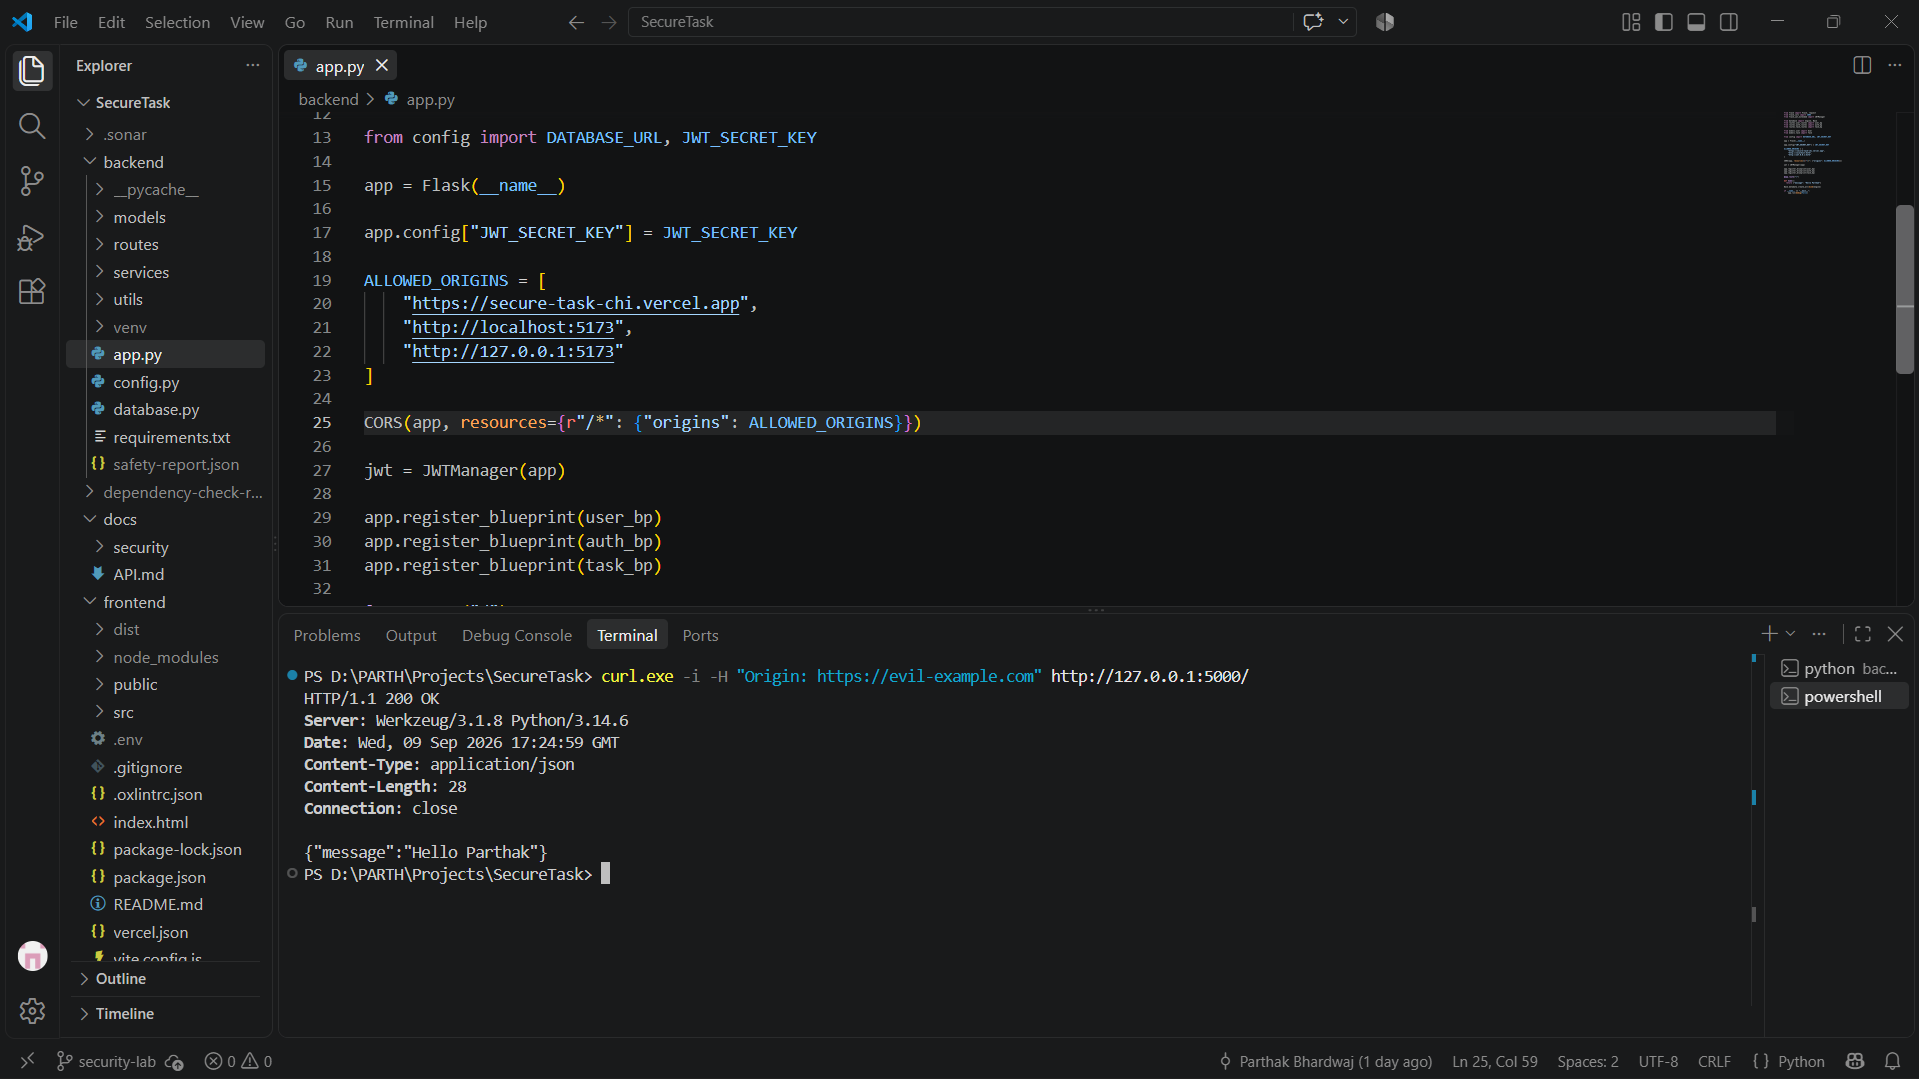
\includegraphics[width=0.88\textwidth,height=0.34\textheight,keepaspectratio]{security/evidence/10-untrusted-origin.png}}{%
    \fbox{\parbox[c][3.2cm][c]{0.85\textwidth}{\centering\color{DarkGray}[Untrusted Origin Test]}}}
  \caption{Untrusted origin CORS verification}\label{fig:cors-bad}
\end{figure}

\subsection{OWASP ZAP Evidence}
\evidence{security/evidence/34-zap-alert-overview.png}{OWASP ZAP alert overview}{OWASP ZAP Alert Overview}
\evidence{security/evidence/41-zap-format-string-root-cause.png}{Manual root-cause analysis of the ZAP password finding}{Bcrypt Root Cause Analysis}
\evidence{security/evidence/42-zap-buffer-overflow-remediated.png}{Bcrypt password-length validation after remediation}{Bcrypt Remediation Verification}

% =========================================================
% 12. FINAL TEST SUMMARY
% =========================================================
\clearpage
\section{Final Security Test Summary}

\begin{table}[htbp]
\centering
\renewcommand{\arraystretch}{1.3}
\begin{tabular}{@{}L{0.5\linewidth}L{0.35\linewidth}@{}}
\toprule
\tablehead \textbf{Test / Check} & \textbf{Status} \\
\midrule
SQL injection & \pass \\
XSS & \pass \\
Authentication bypass & \pass \\
IDOR / authorization & \pass \\
Password hashing & \pass \\
Invalid task ID & \pass \\
Malformed JSON & \pass \\
Verbose error handling & \pass \\
\midrule
Bandit & \pass \\
Semgrep & \pass \\
Gitleaks & \pass \\
Dependency-Check & \pass \\
pip-audit & \pass \\
Safety requirements check & \pass \\
SonarQube & \passcav \\
Bcrypt remediation & \pass \\
Full post-fix ZAP scan & \notdone \\
\bottomrule
\end{tabular}
\caption{Final security testing summary}
\end{table}

% =========================================================
% 13. DEPLOYMENT
% =========================================================
\section{Deployment}

\begin{tabularx}{\linewidth}{@{}L{0.2\linewidth}X@{}}
\textbf{Frontend} & \url{https://secure-task-chi.vercel.app} \\
\textbf{Backend} & \url{https://securetask-backend.onrender.com} \\
\textbf{Database} & Neon PostgreSQL \\
\end{tabularx}

\vspace{0.4cm}
\begin{figure}[H]
\centering
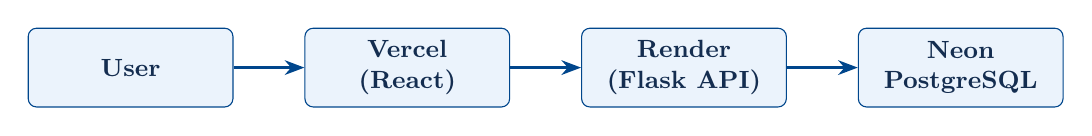
\begin{tikzpicture}[node distance=0.9cm]
\node[flow] (u) {User};
\node[flow, right=of u] (v) {Vercel\\(React)};
\node[flow, right=of v] (r) {Render\\(Flask API)};
\node[flow, right=of r] (n) {Neon\\PostgreSQL};
\draw[arr] (u)--(v);
\draw[arr] (v)--(r);
\draw[arr] (r)--(n);
\end{tikzpicture}
\caption{Production request flow}
\end{figure}

% =========================================================
% 14. CONCLUSION
% =========================================================
\section{Conclusion}

SecureTask combines full-stack development with a structured security assessment. The project delivered a React and Flask application backed by PostgreSQL, with JWT authentication, bcrypt password protection, authorization, protected routes and a live deployment.

Manual techniques and eight automated tools were used to find issues, and several were remediated and re-verified: insecure CORS, a vulnerable dependency, a hardcoded test secret, debug configuration and missing bcrypt length validation.

The project shows the value of pairing automated scanning with manual investigation, remediation and verification, as the ZAP bcrypt finding illustrates.

% =========================================================
% 15. PROJECT LINKS
% =========================================================
\section{Project Links}

\begin{tabularx}{\linewidth}{@{}L{0.25\linewidth}X@{}}
\textbf{GitHub} & \url{https://github.com/bhardwajparthirl/SecureTask} \\
\textbf{Frontend} & \url{https://secure-task-chi.vercel.app} \\
\textbf{Backend} & \url{https://securetask-backend.onrender.com} \\
\end{tabularx}

\end{document}
